\documentclass[12pt]{extarticle}
\usepackage[utf8]{inputenc}
\usepackage[english]{babel}
\usepackage{graphicx}
\usepackage{listings}

% \setlength{\parindent}{4em}
% \setlength{\parskip}{1em}

\renewcommand{\baselinestretch}{2.0}
\begin{document}

\title {How to minimize a function using the Pytorch library \date{} }
\maketitle 

\begin{figure}[h]
\centering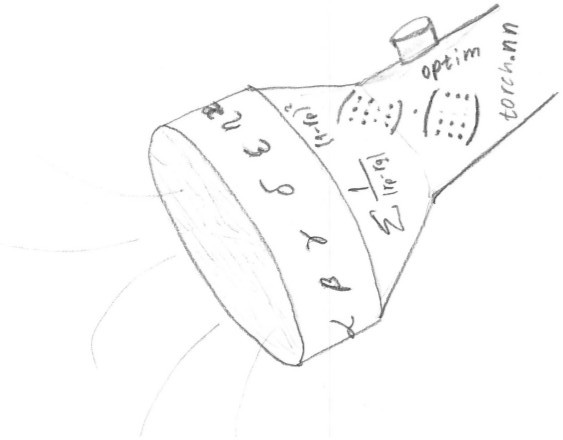
\includegraphics[width=.5\hsize]{pics/magic_torch.jpeg}
%\caption{Extra Boost: an ensemble of gradient boosted trees with extrapolation.}%\ourtitle
\end{figure}


You are now reading the second part of series devoted to
function minimization using the Tensorflow and Pytorch libraries. 
%
The first part shows how to calculate the potential function
of the material points that are attracted to the surface of the unit
sphere, but repelled from each other by the Coulomb force.
%
Here we are going to discuss how to minimize this function using
the Pytorch library.

\section{The Sudden Rakes}

\lstset{language=Python}

Let us discuss the pitfalls that an unaware data scientist can come across using the
Pytorch and Tensorflow libraries.
%
There is a convenient idiom to describe such type of pitfalls.
%
One can call them '''rakes``` because if you face 
one of these problems, it can be painful just as when you step on a rake 
and it hits you on your forehead.
%
Let us discuss rakes that lei on the road of a pure unaware
data scientist.
%
I spent several days trying to find a way to avoid them.
%
Let us repeat the steps from the previous chapter.
%
Throw randomly five points inside the unit cube:
\begin{lstlisting}[frame=single]
import torch
n = 5
k = 1000
torch_coords_np = np.random.rand(n, 3)
\end{lstlisting}
%
Create the tensor - the Pytorch library object that will be changed
during the minimization process:
\begin{lstlisting}[frame=single]
torch_coords_tensor = torch.from_numpy(torch_coords_np)
\end{lstlisting}
%
Then create the wrapper that allows our algorithm to change
the tensor.
%
This wrapper has an effect which is very similar to passing parameters
using pointer or reference semantic in C++ programming language.
%
\begin{lstlisting}[frame=single]
 pt_X = torch.nn.Parameter(torch_coords_tensor)
\end{lstlisting}
%
And, finally, let us put our foot on the rake:
%
\begin{lstlisting}[frame=single]
def create_loss_rake(pt_X):
    pt_xxt = pt_X.mm(pt_X.transpose(0, 1))
    pt_pp_sq_dist = pt_xxt.diag()
    pt_p_roll = pt_pp_sq_dist.repeat(n, 1)
    pt_q_roll = pt_pp_sq_dist.reshape(-1, 1).repeat(1, n)
    pt_pq_sq_dist = pt_p_roll + pt_q_roll - 2 * pt_xxt 
    pt_pq_dist = pt_pq_sq_dist.sqrt()
    pt_pp_dist = pt_pp_sq_dist.sqrt()
    pt_surface_dist_sq = torch.eye(n, dtype=torch.float64) +\
        (pt_pp_dist - torch.ones(n, dtype=torch.float64)) ** 2
    pt_rec_pq_dist = 1 / pt_pq_dist - torch.eye(n, dtype=torch.float64)
    pt_ans_00 = pt_rec_pq_dist.sum()
    pt_ans_01 = k * pt_surface_dist_sq.sum()
    pt_L = (pt_ans_00 / 2 + pt_ans_01) / n
    return pt_L
\end{lstlisting}
%
Actually, we already have some trouble.
%
The handle of the rake speeds inevitably toward our forehead.
%
But there is no impact yet.
%
In order to reveal our problems at full extent, we need to
perform two more steps.
%
Calculate the loss function
\begin{lstlisting}[frame=single]
L = create_loss_rake(pt_X)
\end{lstlisting}
%
And then calculate the derivatives of this function by the parameters
%
\begin{lstlisting}[frame=single]
L.backward()
\end{lstlisting}
%
Let's check the values of the gradient
\begin{figure}[h]
\centering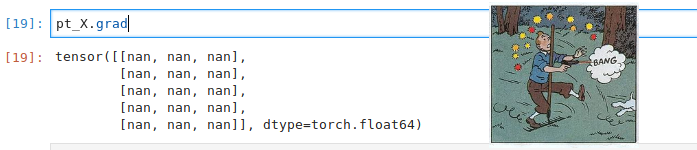
\includegraphics[width=.99\hsize]{pics/rakes_grad.png}
%\caption{Extra Boost: an ensemble of gradient boosted trees with extrapolation.}%\ourtitle
\end{figure}

It is a full \textbf{nan}otechnological success.
%
But what is the reason of our problems?
%
It seems that the only place where we could have problems such as division by zero and, consequently,
\(nan\) values is the calculation of reciprocial
values during electrostatic potential evaluation:
\begin{lstlisting}[frame=single]
1 / pt_pq_dist
\end{lstlisting}
%
But how is it possible, if we added the unit matrix, replacing all
''0`` in \(pt\_pq\_sq\_dist\) to ''1``?
%
Turns out that the values of the function is not the only
thing we ought to care about when we are working  % to take care of 
with the Pytorch and Tensorflow libraries.
%
These libraries use the backward propagation method in order
to calculate the gradient of a loss function.
%
The calculation of a gradient means calculation of a derivative  % to calculate a gradient means to calculate a derivative
for any operation involved in our expression, so it is
necessary to track not only the function scope, but
that of all derivatives inside our function.
%
Looking from this perspective, it is easy to find
the flow in our program.
%
Indeed, one of the operations in our formula is
the square root.
%
The derivative of the square root function is
\begin{equation}
 \left ( \sqrt x \right )' = \frac 1 {2\cdot \sqrt x}
\end{equation}
%
Now it is quite obvious that zeros on the matrix diagonal
cause a division by zero error on the backward propagation step.
%
The solution of this problem is quite straightforward as well.
%
All we need is to place the increase of diagonal elements by one
above the previous line.
%
Let's check what is going on now:
\begin{lstlisting}[frame=single]
 > pt_X.gradient
tensor([[ 29.5873,  11.8047,  18.2031],
        [ 24.6431,   4.5842,  38.6982],
        [ 54.9100,  96.8913,  77.2333],
        [101.3414, 122.9962,  93.9065],
        [-12.4928, -91.3555, -97.1234]], dtype=torch.float64)
\end{lstlisting}
%
Congratulations!
%
This is the gradient matrix. 
%
It shows the direction of maximal growth of our loss function.
%
In the next chapter we will go in the opposite direction 
in order to minimize the value of the loss function.

\end{document}

